\documentclass[border=4pt,dvisvgm]{standalone}
\usepackage{tikz}
\usetikzlibrary{arrows.meta,positioning,shapes.geometric,fit,calc,backgrounds}
\begin{document}
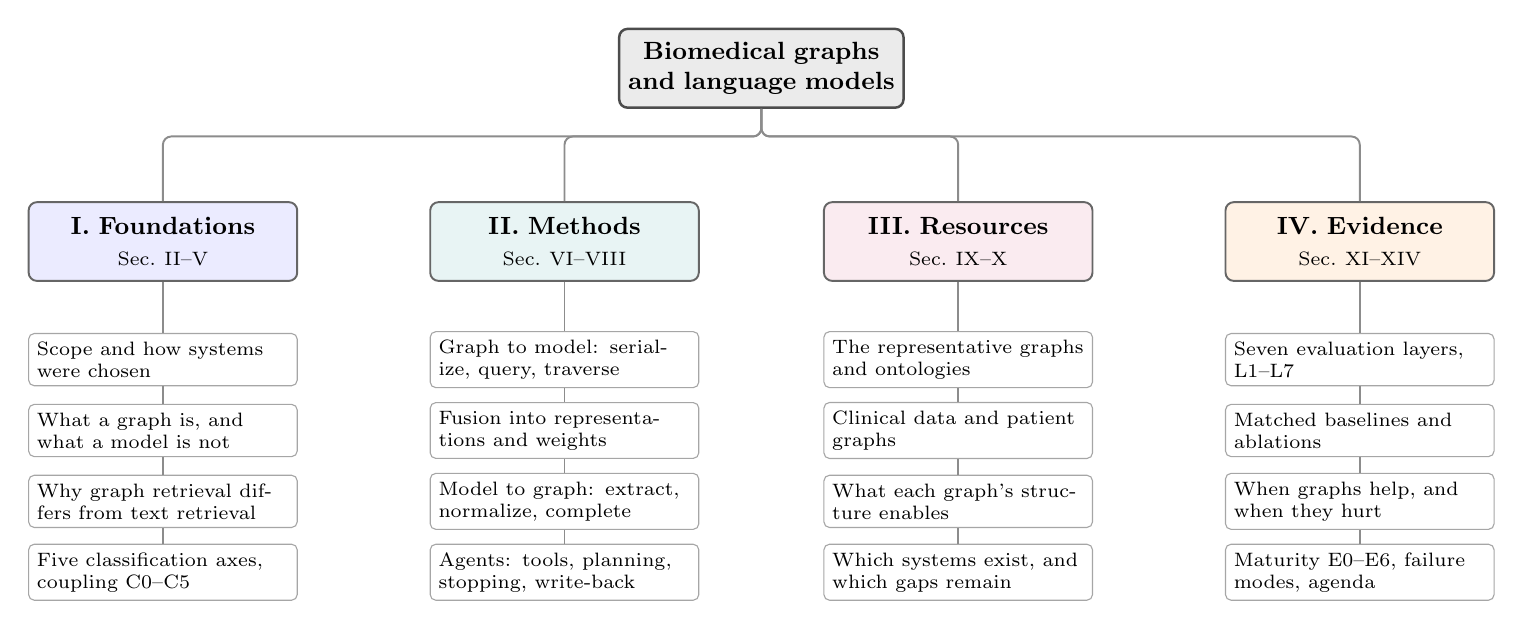
\begin{tikzpicture}[
  font=\small,
  root/.style={draw=black!70, rounded corners=3pt, fill=black!8, text width=34mm,
               align=center, minimum height=10mm, inner sep=3pt, line width=0.9pt},
  part/.style={draw=black!60, rounded corners=3pt, text width=32mm,
               align=center, minimum height=10mm, inner sep=3pt, line width=0.7pt},
  pA/.style={part, fill=blue!8},
  pB/.style={part, fill=teal!9},
  pC/.style={part, fill=purple!8},
  pD/.style={part, fill=orange!10},
  leaf/.style={draw=black!35, rounded corners=2pt, fill=white, text width=32mm,
               align=left, inner sep=3pt, font=\scriptsize},
  e/.style={draw=black!45, line width=0.7pt, rounded corners=3pt}
]

% root
\node[root] (root) at (7.6,1.6) {\textbf{Biomedical graphs and language models}};

% four parts
\node[pA] (p1) at (0,-0.6)    {\textbf{I. Foundations}\\{\scriptsize Sec.~II--V}};
\node[pB] (p2) at (5.1,-0.6)  {\textbf{II. Methods}\\{\scriptsize Sec.~VI--VIII}};
\node[pC] (p3) at (10.1,-0.6) {\textbf{III. Resources}\\{\scriptsize Sec.~IX--X}};
\node[pD] (p4) at (15.2,-0.6) {\textbf{IV. Evidence}\\{\scriptsize Sec.~XI--XIV}};

\draw[e] (root.south) -- ++(0,-0.35) -| (p1.north);
\draw[e] (root.south) -- ++(0,-0.35) -| (p2.north);
\draw[e] (root.south) -- ++(0,-0.35) -| (p3.north);
\draw[e] (root.south) -- ++(0,-0.35) -| (p4.north);

% leaves under part I
\node[leaf] (l1a) at (0,-2.1) {Scope and how systems were chosen};
\node[leaf] (l1b) at (0,-3.0) {What a graph is, and what a model is not};
\node[leaf] (l1c) at (0,-3.9) {Why graph retrieval differs from text retrieval};
\node[leaf] (l1d) at (0,-4.8) {Five classification axes, coupling C0--C5};

% leaves under part II
\node[leaf] (l2a) at (5.1,-2.1) {Graph to model: serialize, query, traverse};
\node[leaf] (l2b) at (5.1,-3.0) {Fusion into representations and weights};
\node[leaf] (l2c) at (5.1,-3.9) {Model to graph: extract, normalize, complete};
\node[leaf] (l2d) at (5.1,-4.8) {Agents: tools, planning, stopping, write-back};

% leaves under part III
\node[leaf] (l3a) at (10.1,-2.1) {The representative graphs and ontologies};
\node[leaf] (l3b) at (10.1,-3.0) {Clinical data and patient graphs};
\node[leaf] (l3c) at (10.1,-3.9) {What each graph's structure enables};
\node[leaf] (l3d) at (10.1,-4.8) {Which systems exist, and which gaps remain};

% leaves under part IV
\node[leaf] (l4a) at (15.2,-2.1) {Seven evaluation layers, L1--L7};
\node[leaf] (l4b) at (15.2,-3.0) {Matched baselines and ablations};
\node[leaf] (l4c) at (15.2,-3.9) {When graphs help, and when they hurt};
\node[leaf] (l4d) at (15.2,-4.8) {Maturity E0--E6, failure modes, agenda};

\foreach \p/\a/\b/\c/\d in {p1/l1a/l1b/l1c/l1d, p2/l2a/l2b/l2c/l2d,
                            p3/l3a/l3b/l3c/l3d, p4/l4a/l4b/l4c/l4d} {
  \draw[e] (\p.south) -- (\a.north);
  \draw[e] (\a.south) -- (\b.north);
  \draw[e] (\b.south) -- (\c.north);
  \draw[e] (\c.south) -- (\d.north);
}
\end{tikzpicture}%
\end{document}
